\ifdefined\included
\else
\setcounter{chapter}{4} 
\dominitoc
\faketableofcontents
\fi

\chapter{User Study to evaluate an integrated plan and execution scheme in simulation}
\chaptermark{Integration and Evaluation of a collaborative scheme}
\label{chap:5}
\minitoc

\section{Introduction}

To validate the approach presented in the previous chapter we conducted a user study on more than twenty participants. The purpose of this study is two-sided. 
First, we want to validate our overall planning approaches based on the proposed Model of Execution, and thus, show how it allows successful collaboration with a human. 
Secondly, we want to validate the Model of Execution itself, that is, showing how it allows the human to always be the leader and able to decide while the robot follows concurrently. We use a simple baseline to compare the Model of Execution with, and we show how our model allows to better satisfy human preferences and thus is preferred. 

\textbf{TODO: Explicit hypothesis? Cronbach’s alpha?}

We decided to conduct this study in simulation for various reasons. First, one of our assumptions is that all actions should roughly have the same duration. However, real-life robots are slow and not very reactive. Those aspects may bias the results of our study which is focused on decision-making. Secondly, simulation allows several simplifications that are acceptable for study. Collision with the cubes has been disabled to make the robot faster both in planning and executing its arm movements. In addition, simulation allows having a perfect perception of the environment. In a real-life experiment, perception errors may occur leading to replan, and thus slower execution, or even wrong decisions. Moreover, our model assumes that both agents synchronize after each step. Hence, it was easy in simulation to prevent the human from acting too soon and synchronize automatically their actions. In a real-life scenario, we couldn't physically prevent the participant from acting. This would imply a heavier training process for the participants to avoid desynchronizing with the robot. In practice, an additional execution supervisor should be developed to permit desynchronizing as long as they are not too big, and hence, prevent the system from crashing. This would require a significant technical effort to implement.

To conduct this study I developed a dedicated interactive simulator using a Tiago robot. In addition, the automaton described by the MoE has been implemented and integrated with the simulator to provide a proper execution and supervision scheme. Eventually, through carefully designed scenarios and using a shortened version of the PeRDITA questionnaire we gathered the feelings and impressions of the participants regarding the different robot behaviors. We also recorded logs from each executed scenario allowing us to draw a timeline of the execution and compute objective metrics for each scenario among which can be found: the time to complete the task, the human reaction time or the time for the human to be free. Several relevant facts and conclusions can be extracted from the collected results and are discussed in this chapter.

This chapter is organized as follows. First, the interactive simulator functionalities and operations are described. Then the methodology of the user study is provided along with anonymous information on the participants. After, the results obtained are presented and then discussed, validating the proposed hypothesis.

****

why simulation: HRI rebuttal: we rely on a reactive execution, real life robot are slow and not very reactive, may have perception errors, thus may bias our results focused on decision making.

Thus, we developed an interactive simulator running robot policies generated as explained the Chapter~\ref{chap:4}. Then, we conducted a user study using this simulator.

The purpose of this study is two-sided. First, we want to validate our overall planning approaches based on the proposed Model of Execution, and thus, show how it allows successful collaboration with a human. Secondly, we want to validate the Model of Execution itself, that is, showing how it allows the human to always be the leader and able to decide while the robot follows concurrently. Compared to a simple baseline, we also want to show how this model allows to better satisfy human preferences and thus is preferred. 

This chapter is organized as follows. First, interactive simulator functionalities and operations are described. After, the study protocol is presented as well as some analysis of the participants. Eventually, the obtained results are presented and discussed.

% *****

% Objective of the study is to validate the following:

% \begin{itemize}
%     \item \textbf{Overall planning and the use of Model of Execution during planning}: Always reach the goal, with different preferences, no need of prior negotiation, overall positive interaction, simple, use of MoE allows to explore all possible execution traces and complete the robot policy allowing human free to choose any action (OptimalRatio < 1.0) while still having a reactive robot, step synchronization questionable (sometimes liked, helps participant. Sometimes a bit lost in the step, however still ok.), real scenario should use additional execution supervisor allowing step superposition.
    
%     \item \textbf{Use of Model of Execution during execution}: The MoE describes how the robot always acts in a concurrent and compliant manner with the human. This allows the human to always (at every step) be in control. By using a mirror baseline where the robot always takes the lead instead of being the follower, we show that having the robot as a follower is preferred (H feels in control) and allows for better satisfying human preferences. The drawback of this approach is that currently, the robot is always a follower, making it slower since it always waits for the human to do something to adapt and act. Given to good results of the RF (with correct estimation) the question arises of trying to mix both approaches, having a robot that is by default a follower but sometimes takes the lead to be faster (when no risk of conflict?)
    
%     \item \textbf{Neither HA-planning nor compliant execution are sufficient alone}: Indeed, when the robot follows the HF regime with an incorrect estimation of human preferences the human can ``impose'' their decisions on the robot which will adapt, and thus, the human can satisfy their preferences anyway. However, in such scenarios, the human usually have one chance to impose their decision. Hence, if they are distracted the robot will eventually act in a not desired way which can lead to negative interaction. This can be observed with some participants either getting confused or distracted, and this didn't happen when the robot had a correct estimation of human preferences. Hence, it is important to have both a pertinent robot policy/plan selection complemented with an adaptive and compliant execution to have the best interaction possible.
    
%     \item \textbf{Not investigated in this work but,} our approach has been designed to allow specifying online new human preferences, updating the whole robot policy to satisfy the new given preferences. This allows either the human to directly specify their intents and preferences to the robot, or, an external process estimating online the human preferences.
% \end{itemize}

% The goal is to validate our approach presented in the previous chapter and justify the following. We believe that the robot should plan its actions with a compromise of optimizing the task efficiency, maximizing social criteria and satisfying human preferences while collaborating with humans. However, satisfying those social criteria is challenging since they cannot be accurately quantified. Especially for human preferences which can fluctuate a lot depending on their mood and context. That is why we believe, in addition to planning the best course of action using all these criteria, it is relevant or even mandatory for the robot to adapt and be compliant with human online decisions and actions. 

% Hence, this study aims to show two main things. First, during execution, the robot should adapt and be compliant with the human actions. Indeed, it is hard to accurately estimate human behavior and preferences. In case of incorrect estimation, having a compliant robot helps to satisfy the human preferences (HF vs RF, better answers). Also, the human may act differently than expected by the robot, the latter should be able to allow this and comply with it (ratio\_h\_optimal < 1.0).
% Secondly, the study validates our overall planning (and execution?) approach. The goal is always solved. The collaboration is always useful (more or less) and not so low (positive). 
% Third, we can also say that despite having to be compliant online, it is very beneficial to plan correctly beforehand the robot actions. 

% \textbf{TODO: GOAL of the study is to validate two things. First, our overall planning approach. Secondly, the HF model of execution. 1) Should see that overall even when wrong RF the robot isn't so bad, still useful, simple, competent, responsive. Could do better and a bit frustrating but still ok to accomplish the task. 2) Should see that HF is significantly preferred and results in more acceptable and appreciated behavior : Adaptive, Appropriate, Accommodating, Positive.}

\section{Related work}

\subsection{Questionnaires}
Many questionnaires are used in the field of HRI. The main ones are listed here: GodSpeed, HRIES, PeRDITA, RoSAS, Trust Perception Scale-HRI. 

Each questionnaire has specificities and helps to measure certain aspects of the robot. Many include appearance items to evaluate the look of the robot. Since our focus is on robot decision-making, we decided to base our questionnaire PeRDITA. Indeed, this questionnaire has been designed to evaluate the pertinence of robot decisions in a Human-Robot Joint Action Context, which is exactly our case. Yet, the full questionnaire is a bit heavy and also covers communication which isn't our topic in this work. 
That is why we decided to shorten the questionnaire by removing the section on communication and a few redundant items. Redundant items are helpful to evaluate the consistency of a questionnaire and this has already been done in~\cite{devin_evaluating_2018}. Hence, to avoid participants getting bored and lost by filling out the whole questionnaire after every scenario we kept 12 items covering the following dimensions: robot perception, interaction, collaboration, and acting.


\section{Interactive Simulator}
planning is same

execution is based on model of execution and mock components

human collaborates in real time with robot in blockwords task

describe simulator, mouse, robot and human capabilities, goal shown, prompt

Synchronization, internal communication through simulated visual signal, explicit reaction time, ID phase currently always successful a success rate can be given. 



***********

In this section we provide a few functional and technical details about the developed interactive simulator used for the User Study, its overall structure is shown on fig~\ref{fig:simu_architecture}.

\begin{figure}
    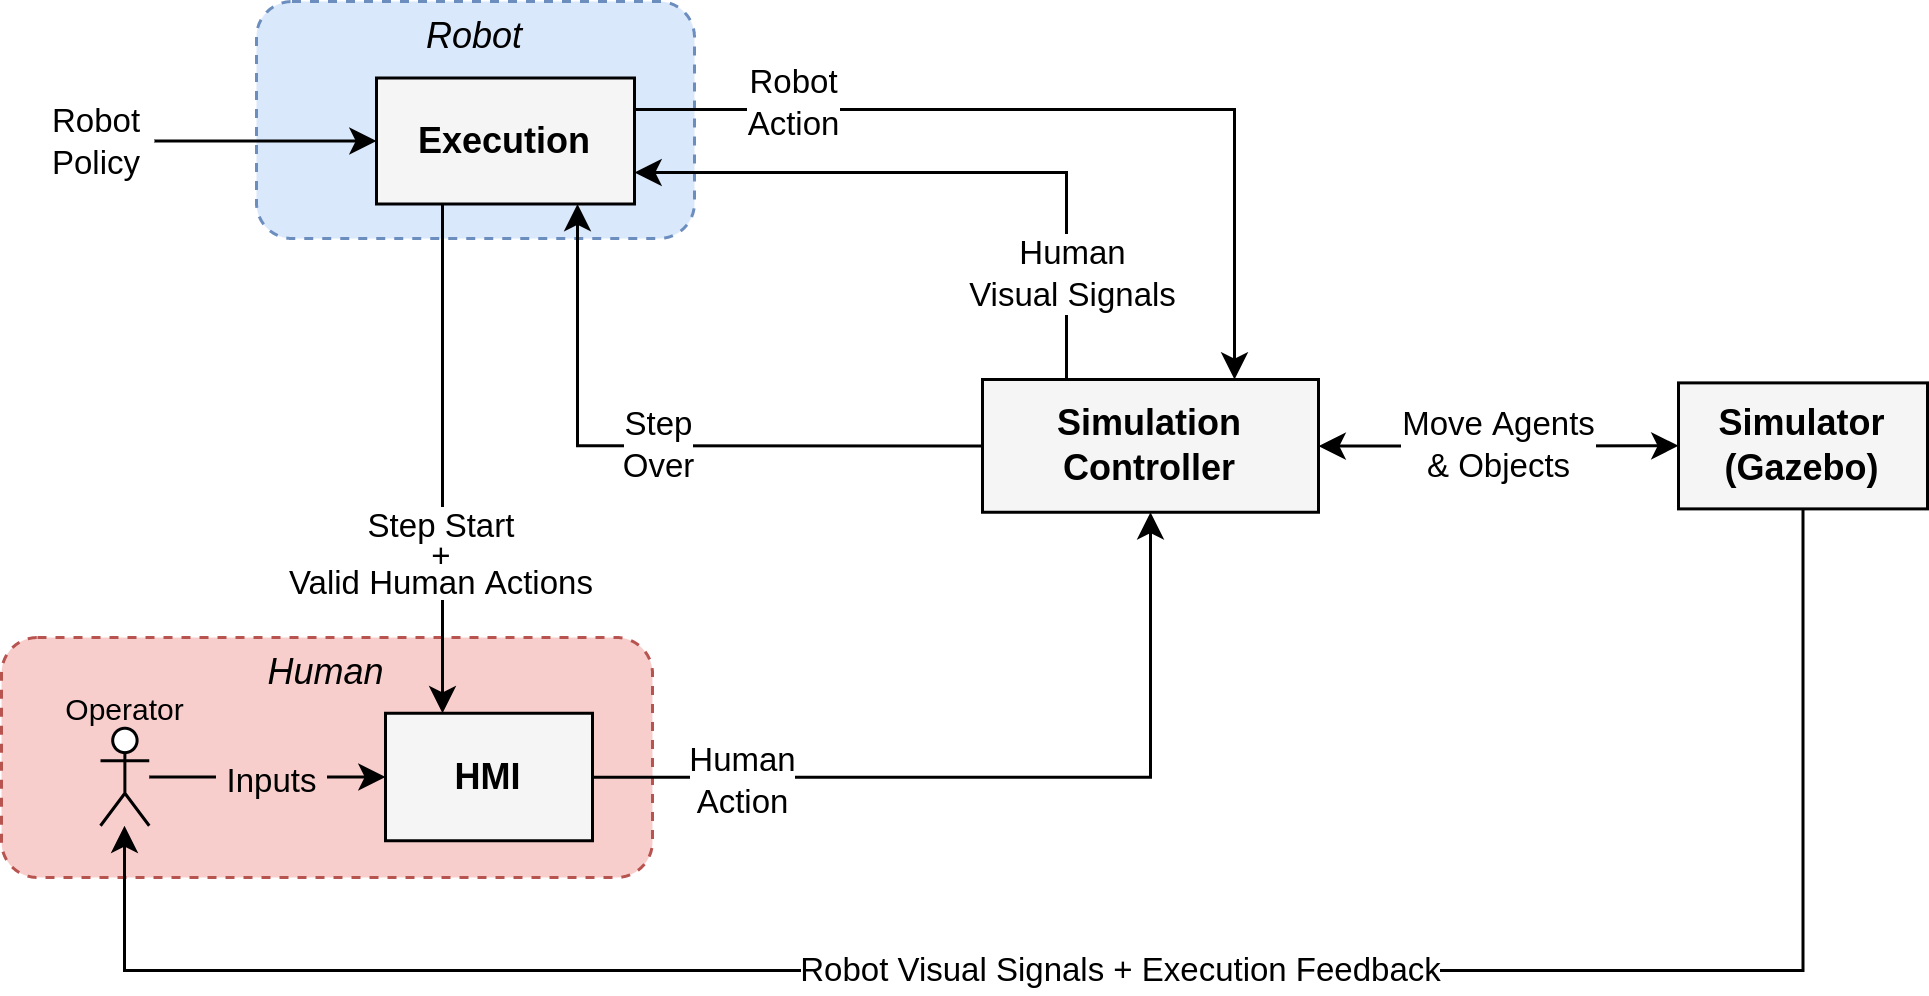
\includegraphics[width=\textwidth]{images/Chapter5/simu_architecture.png}
    \caption{Overview of the Interactive Simulator's Architecture}
    \label{fig:simu_architecture}
\end{figure}

\begin{figure}
    \centering
    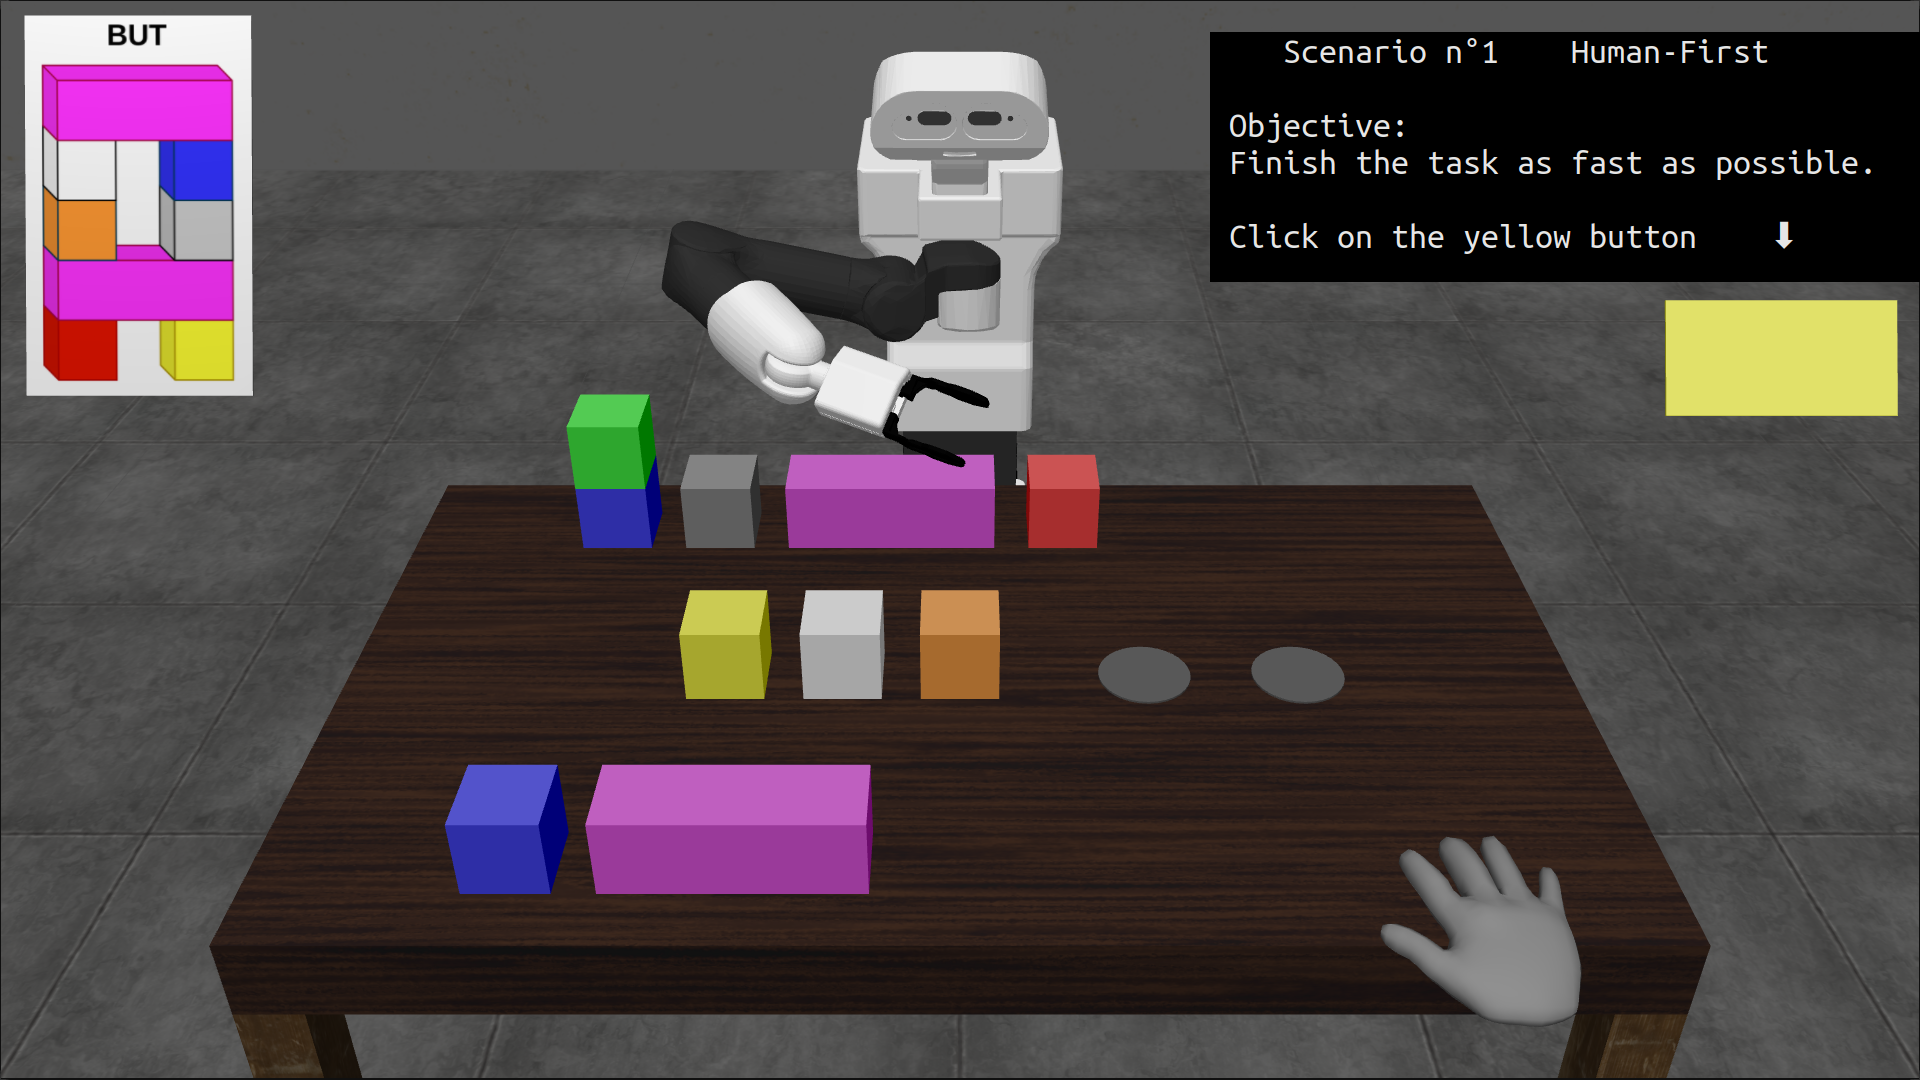
\includegraphics[width=\textwidth]{images/Chapter5/simu_screenshot.png}
    \caption{Participant view of the interactive simulator. Text prompt. Goal pattern. robot. table. cubes. stacking area. human hand.}
    \label{fig:simu_view}
\end{figure}

First, it is using Gazebo to simulate the scene (table, cubes, agents). 
The robot is a Tiago robot from PAL Robotics. We used a MoveIt controller to plan and execute arm motions. We used a publicly available component to control the gaze of the robot. The head behavior is ad hoc and designed by us.
The human agent is simulated only with its hand which is moved with a handmade dedicated controller. 
For simplicity reasons physics of objects isn't simulated, thus, each agent interact with the scene by statically attaching/detaching object respectively to the robot's gripper or the human hand.
A higher level component called the simulator controller is in charge of translating primitive actions to low level commands and calling the previously presented controllers to make the agent perform actions. Since it manages agent's action, it is also in charge of sending simulated visual signals and indicating when a step is over. Indeed, the agents synchronize themselves using simulated visual signals, and not internal signals. That is, when the human starts performing an action, a brief motion planning phase occur before effectively moving the hand, the motion visual signal is sent to the robot only at this moment. Moreover, to simulate some real perception aspect, a voluntary reaction time is introduced in the robot. Thus, the visual signal can be treated only after this reaction time is passed. A step starts when one agent starts acting (the human or the robot) and it is over when both agents are inactive. Hence, once one agent started to act the other is free to perform an action concurrently and the step will be over only when both are done. If the other agent doesn't act it will be considered as passive/inactive and the step will be over as soon as the first agent finishes.

Then we can find the respective agents' components. The robot component is an implemented version of the model of execution. Its purpose is to supervise the policy execution of the robot while running the automaton described in the model of execution. In practice, the robot starts by indicating when the step started with a sound signal. Then, it waits to receive the visual human signals for a defined amount of time. Without any visual signal the human is considered as passive. The human can either start acting (how will be described just after), which will eventually send a visual signal to the robot, or the human can make an explicit hand gesture to indicate to the robot that they will be passive (this doesn't force the human to be passive for the whole step). Note that even if the robot received the human visual signal of the human starting to act, the actual action being performed isn't yet identified, it only means that the human started to act. The robot must perform a dedicated identification process (ID Phase/Process) to identify the human action. We assume that the hand gesture that the human can make is always successfully identified instantly (without ID Process). Once either the signal received or the time-out reached, if the best robot action doesn't depend on the human decision then the robot can directly start executing this action. The robot action choice is sent to the simulator controller that will start executing the action. If the best robot action depends on the human decision then the human decision must be identified and the ID Process is run. Only after the robot can perform the best action indicated by the policy which is compliant with the identified human action. If the ID Process fails then the robot remains passive, this case is already part of the policy.
Eventually the robot waits for the step over signal from the simulator controller and run the Assessment Process. The latter identify what happened during the step (which action the human performed, even if ID wasn't necessary) and in which state we are to be ready to execute the next step and progress in the policy and toward the goal. 

The human action execution consists in the following. First, the gazebo simulator is made as the main Human-Machine Interface (HMI). Through a handmade plugin one can mouse click in the gazebo simulator window. The click position is sent on a ROS Topic and treated in a dedicated node to potentially trigger a human action. For instance, clicking on a cube starts a "picking" action with the corresponding cube as parameter, clicking on the stack area starts a "place" action, clicking on the table while holding a cube starts a "hold" action, and clicking on the hand make an explicit hand gesture to signal the robot the human desire to be passive. After clicking the hand once, the participant can click another time to indicate the robot full passivity until further notice. The robot will consider the human as unavailable or even not present and will not wait for them. 
For this to be possible we did the following. First, another gazebo plugin has been written to lock the GUI camera as a First Person View and avoid the participant to accidentally move the camera.
Then, at every step, the robot component sends to the component receiving the coordinates of the click the currently valid human actions that the participant can perform. Thus, the participant cannot try to place a cube without holding it. Eventually, each human action is mapped to a clickable zone on the gazebo window. Hence, when the click coordinates are received, we check if it is inside one of the designed zone and is the action associated to the zone is currently valid. If so, then the action decision is sent to the simulator controller to be executed. 
For clarification purpose, when clicking on a cube the robot doesn't immediately know that the human is picking a cube. First, it will know that the human started to act only after receiving the visual signal (after the defined reaction time). And the robot must perform an additional perception phase (ID Process) to identify which action the human performed. 

Additionally, the stacking goal pattern is shown inside the simulator and a small prompt overlay is present to simulate a potential screen with which the robot can communicate its intention to the human during the collaboration. 

Thanks to all these processes, the participant is able to intuitively perform actions using mouse control and can collaborate with the robot to solve the task.

An integrated tutorial has been made to familiarize the participant with the mouse control and the relevant concepts used in the collaboration (notion of step, able to be passive). 

\section{Study protocol}

Methodology: 
Initial demographics' questionnaire to identify potential individual difference ratings. Then, presentation instructions/text. After, familiarized with simulator through an interactive tutorial. Eventually, the six scenarios in randomized order are experienced by the participant. After each scenario the participant answers a shortened version of the PeRDITA questionnaire and logs about the execution are saved. Eventually, the participant is asked about their overall impressions regarding the interaction they had with the simulated robot, and they are asked which scenario they preferred the most and the least. 

objective, participants, material, experiment design, procedure, measures

This section describes the objectives and protocol of this study.  



\begin{figure}
    \centering
    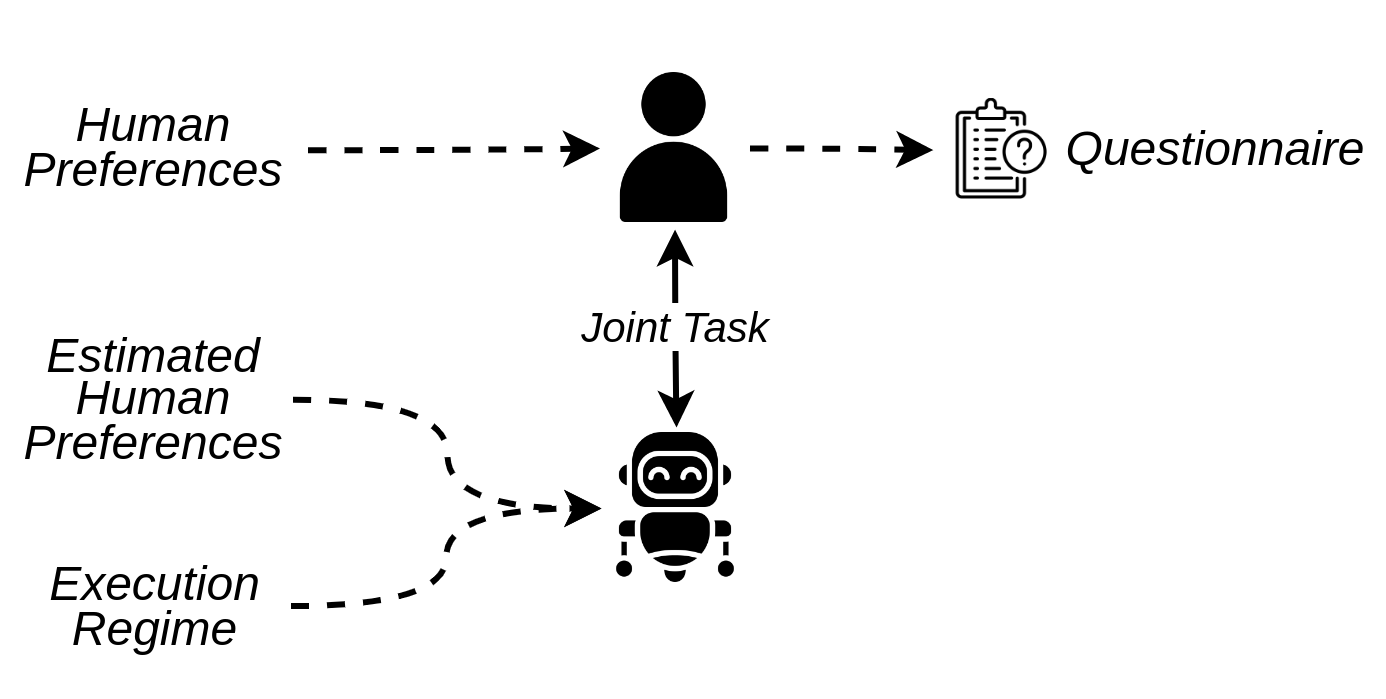
\includegraphics[width=0.8\textwidth]{images/Chapter5/UserStudyProcedure.png}
    \caption{A scenario of the User Study Protocol. Each participant goes through 6 scenarios and answer 6 questionnaires to evaluate each different robot behavior}
    \label{fig:user_study_protocol}
\end{figure}




Through this study we want to demonstrate the benefits of using the model of execution described in the previous chapter~\ref{chap:4} in a collaborative context. We believe this model of execution is pertinent to be taken into account when executing and supervising a robot's plan. For the same reasons we based the policy generation of this model and aim to justify our choice and validate our approach.

In this study, each participant is made to collaborate six times with a simulated robot to achieve a shared task, each time is referred to as a scenario. The robot exhibits a different behavior in each scenario. After each scenario, the participant evaluate the robot's behavior through the PeRDITA questionnaire \cite{devin_evaluating_2018}.

Beforehand, every participant answers a few general/demographic questions and is familiarized with the simulator functionalities through an integrated tutorial. Only then they start the six consecutive collaborative scenarios, answering every time a questionnaire to describe the interaction. Eventually, every participant is asked to share their general feelings and impressions about the overall interaction with the simulated robot, and they are asked to tell which scenario they preferred the most and the least.

\begin{figure}
    \centering
    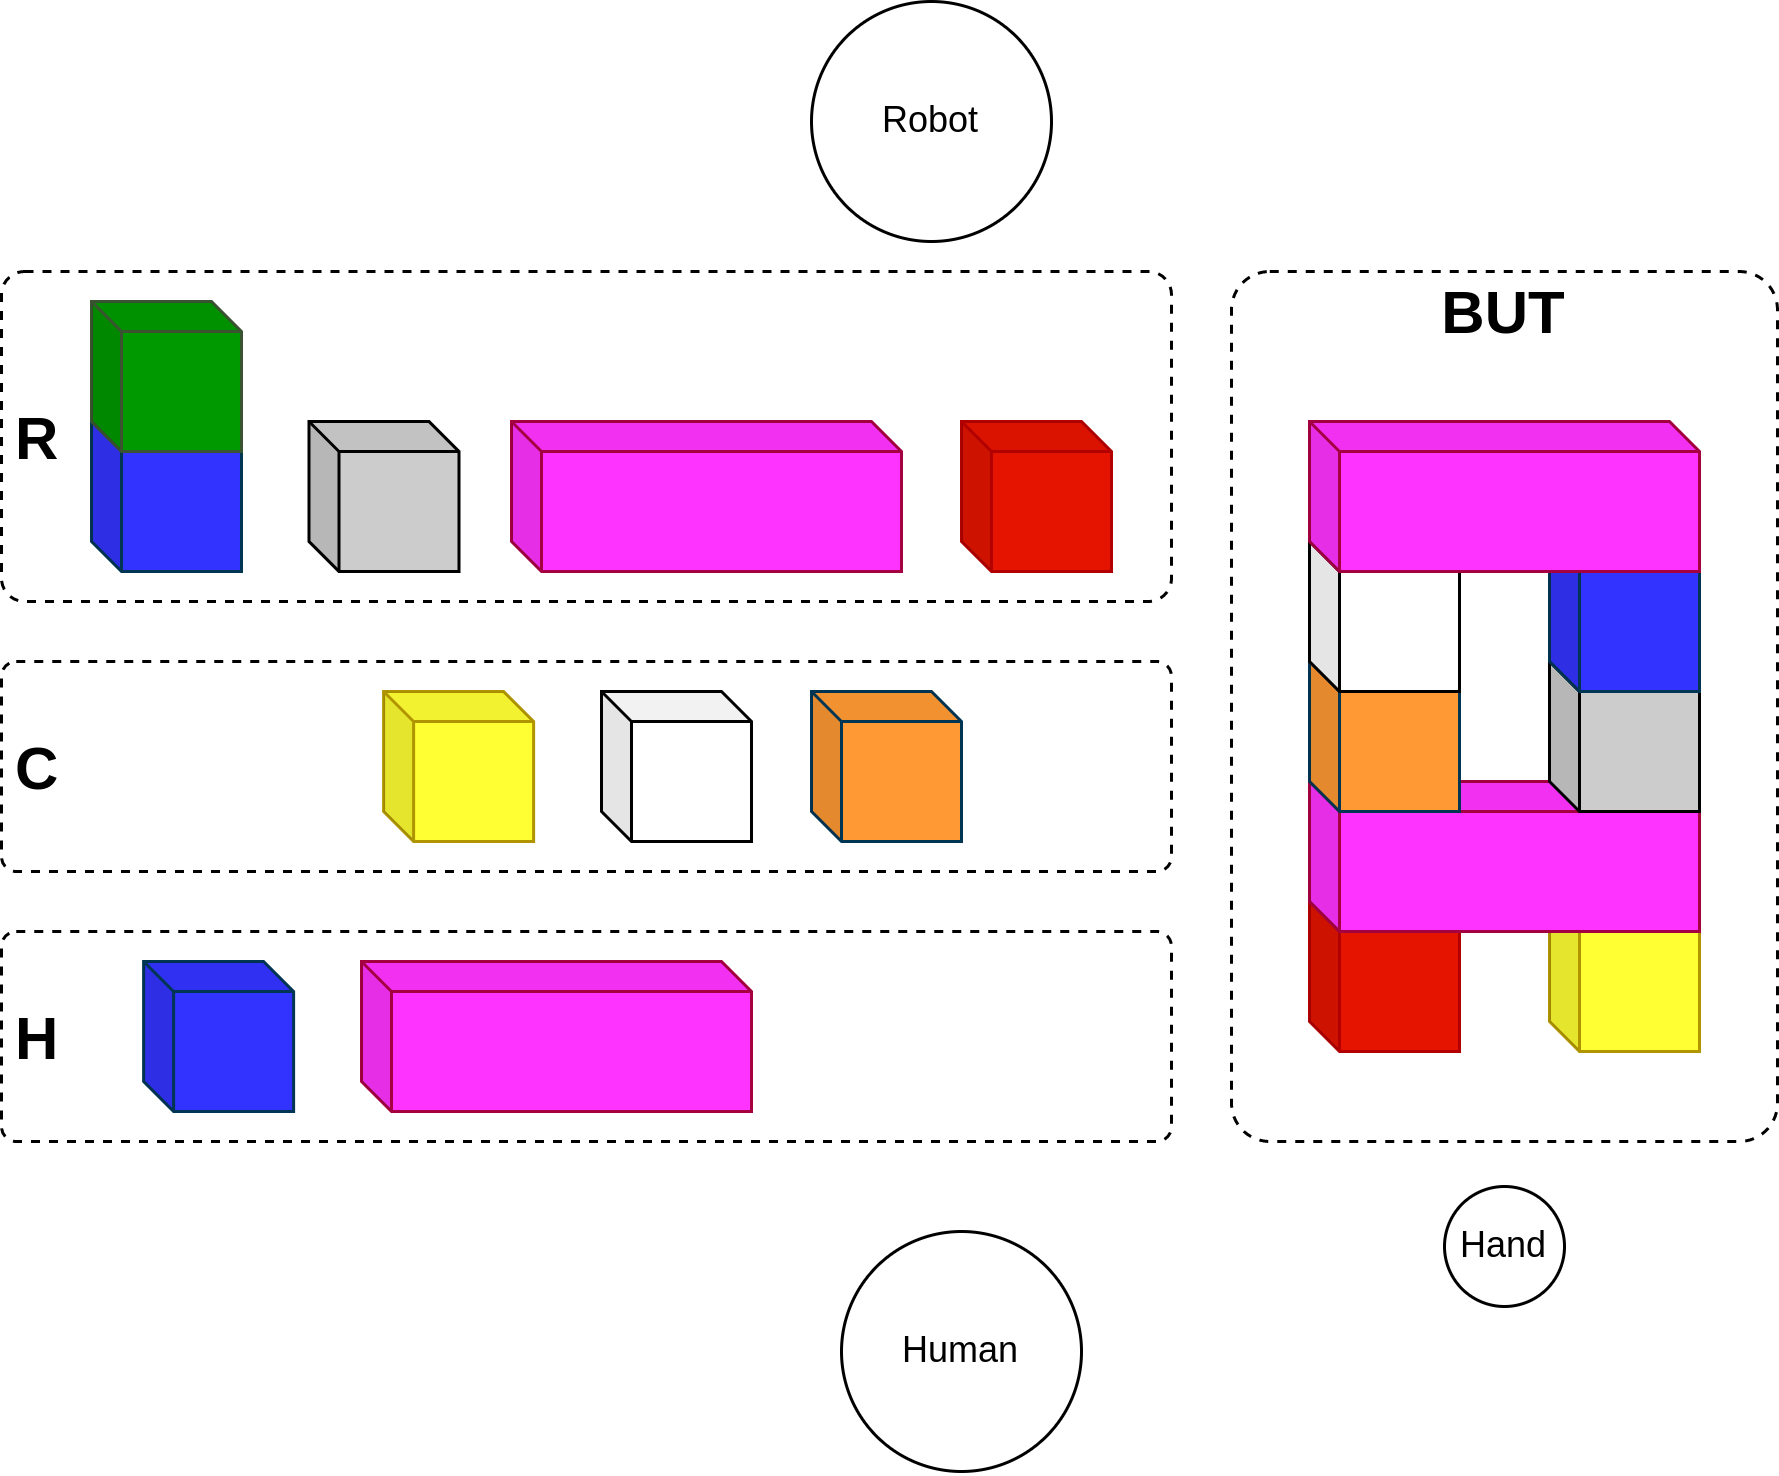
\includegraphics[width=0.8\linewidth]{images/Chapter5/task_description_study.png}
    \caption{Description of the shared task to achieve in the study.}
    \label{fig:task_description_study}
\end{figure}

We now provide details about the task, the scenarios and how the different robot behavior are generated. 
The shared goal, which is stacking the cubes to match the given pattern, remains the same in all scenarios. The cube disposition on the table also doesn't change either. The task description is depicted in fig~\ref{fig:task_description_study}. 

To progress in the task, the agents can perform three different primitive actions which are the following: \textit{pick} a cube, \textit{place} a cube in the stack, or, \textit{drop} a cube back on the table.
These actions have a few preconditions, more or less intuitive, that are communicated and experienced by the participant during the integrated tutorial.
First, one can \textit{place} a cube if they hold the cube, and if the targeted location is free and supported. That is, the cubes directly below the targeted location must be placed before being able to place a cube in the targeted location.
Secondly, one can only \textit{pick} a cube from their respective reachable zones of the table, i.e., Human and Center zones for the human, and Robot and Center zones for the robot. Also, one can only pick a cube if it can be placed immediately. Thus, one cannot pick a cube ``in advance'' and has to wait to its placement condition to be true before picking it up. For instance, both pick bars can only be picked up after the yellow and red cubes have been placed. This rule helps to create interaction conflicts serving the purpose of this study. Moreover, although the participants find this not intuitive they get used to it really fast and this feeling seems to be significantly reduced along the experiment.
Third, one can \textit{drop} a cube back on the table only if they hold it and if it cannot be placed.

For each scenario the participant is given instructions regarding how to solve the task. The participants are asked to consider these instructions as their own choice and preferences regarding the task resolution, and thus, to act accordingly while collaborating. The instructions at each scenario are one of the two following.
On the first hand, the participant shall act in a way to finish the task as soon as possible. Here, it consists in trying to perform as many actions in parallel as possible to progress faster. These preferences are latter referred to as Task End Early (TEE).
On the other hand, the participant shall act in a way to be freed as soon as possible. That is, they should finish their mandatory part of the task as soon as possible, so they could leave and let the robot finish alone. Here it consists in placing the pink bar from the Human zone as soon as possible. These preferences are latter referred to as Human Free Early (HFE).
On its side, the robot doesn't directly have access to these instructions/preferences, they are only estimated. Hence, for each scenario, the robot is given a more or less accurate estimation of the human preferences that are communicated to the participant. Note that the participants aren't aware that the robot has an estimation of their preferences, neither that this estimation can be inaccurate.
This way, we created three scenarios with different pairs of human preferences and associated estimation. In the first pair, the human shall finish the task early and the robot has a correct estimation, i.e., the robot's policy is helping the human to finish the collaborative task early. In the second pair, the human preferences remain the same, but the robot estimation is incorrect. The robot is trying, mistakenly, to minimize the human effort. As a consequence, the robot tends to pick cubes that the human could pick, preventing the human from acting and making the task completion longer. In the third pair, the human shall free themselves early, but the robot estimation is again erroneous. The robot will try to finish the task early while its priority is to place the first pink bar, which is conflicting with the given human preferences.

Additionally, in each scenario, the robot follow one of the two following execution regimes:
\begin{itemize}
    \item \textbf{Robot-First (RF)}: the robot always initiates actions first, and the participant take action afterwards.
    \item \textbf{Human-First (HF)}: the robot always lets the participant take the initiative, and then acts.
\end{itemize}
The \textit{Human-First} execution regime corresponds to the Model of Execution described in the previous chapter. At each step, the robot waits for the human's decision and will execute the best action that complies with it. The human always start acting first and the robot follows. On the other hand, the \textit{Robot-First} regime corresponds to a naive and straightforward policy execution where, at each step, the robot directly starts executing the overall best robot action given by the policy. The robot always starts acting forcing the human to comply. The \textit{Robot-First} regime serves as a baseline to evaluate the proposed \textit{Human-First} regime, described by our Model of Execution and used in the policy generation.
Eventually, we associate each of the three previous pairs of preferences and estimation with one of the two different execution regime. As a result, we obtain six different scenarios with six different robot behaviors named in table~\ref{tab:scenario_names}.

\begin{table}
    \caption{Name of the six scenarios. 
    Columns represent the preferences/estimation pairs and the rows correspond to the execution regimes.}
    % \vspace{-15pt}
    \begin{center}
    \begin{tabular}{c|c|c|c|}
        \cline{2-4}
                                                & Pair A        & Pair B            & Pair C\\
                                                & TEE: correct  & TEE: incorrect    & HFE: incorrect\\
        \hline
        \multicolumn{1}{|c|}{Human-First}       & S1            & S3                & S5\\
        \hline
        \multicolumn{1}{|c|}{Robot-First}       & S2            & S4                & S6\\
        \hline
    \end{tabular}
    \end{center}
    \label{tab:scenario_names}
\end{table}

Note that our goal is to evaluate and compare the different robot behaviors. However, at the beginning, the participants don't have any references to compare with which can influence their answers in the very first scenarios. One solution is to ask the participants to answer all six questionnaires at the end, after being familiar with the six scenarios. We consider that this option demands a too heavy mental workload to recall accurately each specific scenario, and may bias the answers. As a consequence, we decided to ask the participants to answer the questionnaire after each scenario as a draft. Along the experiment, they can rectify their answers to match more accurately their feelings. At the end, using the drafts, they share their final answers for each scenario. We believe this process allow to more accurately gather the feelings of the participants. Moreover, the ordering in which the participants encounter the scenarios is uniformly randomized to prevent any order effect. 

\textbf{TODO: Give more details about the PeRDITA questionnaire (questions, goal, etc..)}

On top of the answered questionnaires, for each scenario, the interactive simulator produces logs from which we extract several metrics and an overall timeline of the execution. The timeline depicts the activities and actions of each agent along the task progression. The subjective measures done through the questionnaire are complemented with the objective metrics extracted such as the duration to complete the task, the number of human action, the total duration of human inactivity, and more. 

Here is an example of a timeline and below the associated extracted metrics:

\begin{figure}
    \centering
    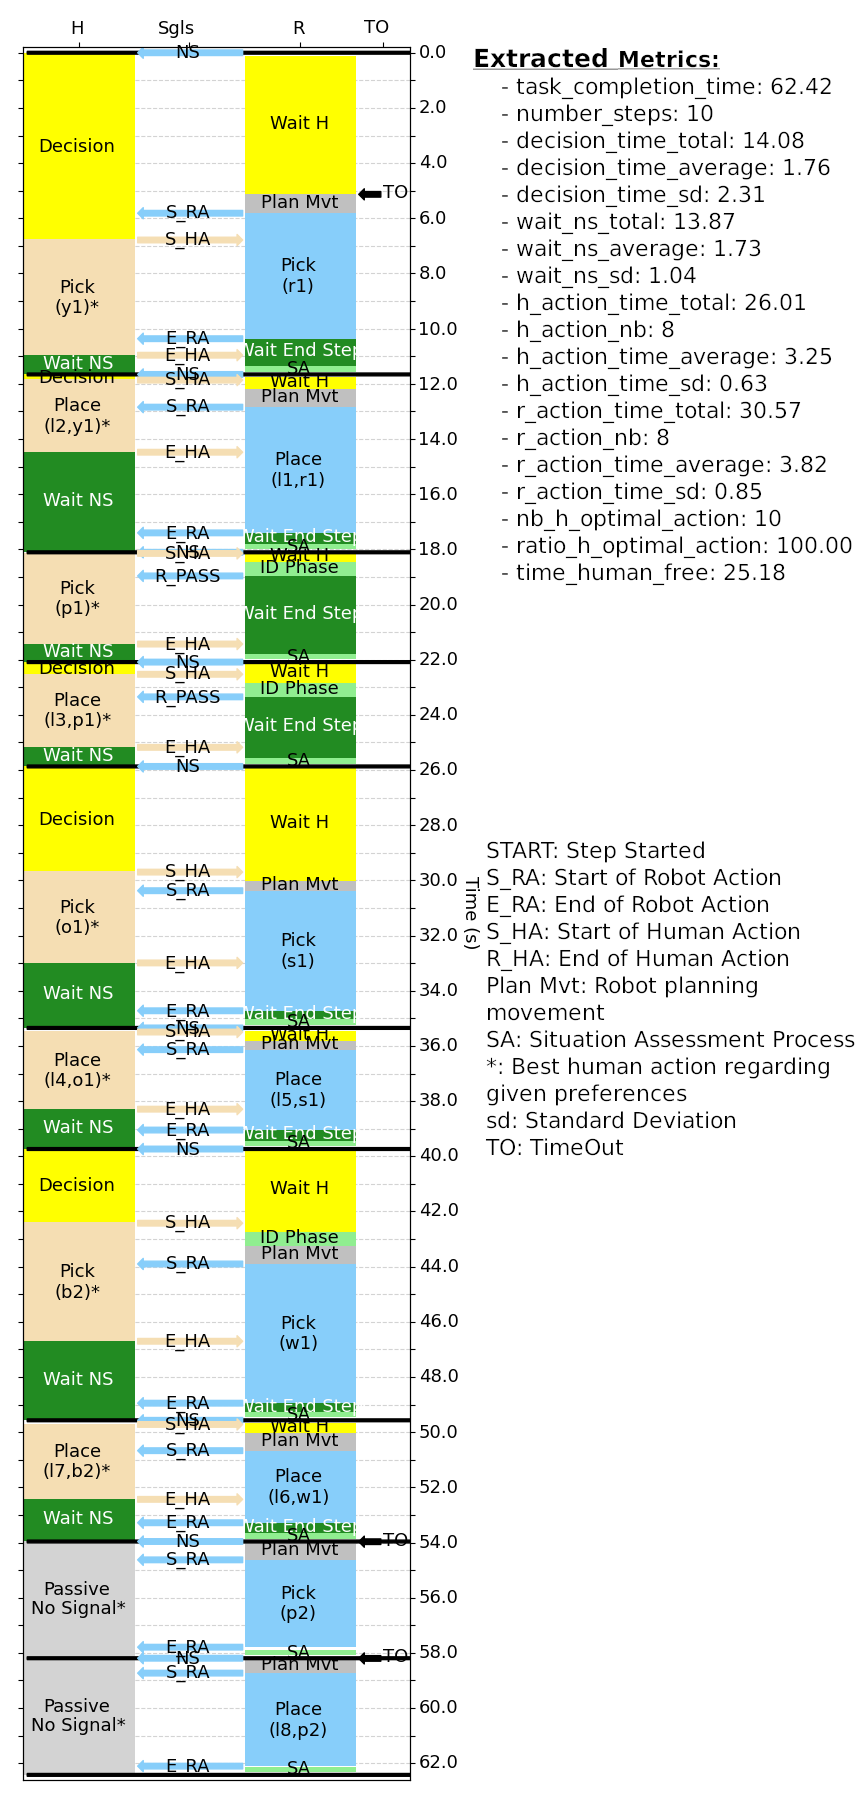
\includegraphics[width=0.73\linewidth]{images/Chapter5/timeline_example.png}
    \caption{Example of a timeline produced by the simulator after a scenario.}
    \label{fig:timeline_example}
\end{figure}





\section{Study results}

% ns  P > 0.05
% *   P ≤ 0.05
% **  P ≤ 0.01
% *** P ≤ 0.001

In this section, we share the main results obtained through the answered questionnaires and the metrics extracted from the logs.

\subsection{Assumptions}

For analysis we rely on ANOVA tests that requires data to follow a normal distribution. 

Here the data, most of the metrics, are close to following a normal distribution (checked using Kolmogorov-Smirnov, Shapiro-Wilk and Anderson-Darling tests). Thus, parametrics tests can be applied, and we used either paired t-tests or ANOVA with repeated measures.

In the last case, Bonferroni Post-hoc-Tests are performed to identify exactly which groups are significantly different from others.



\subsection{From timeline}
\textbf{TODO: For now with only 9 participants, it is hard to extract any relevant result from the logs. The timelines vary considerably. So far, we can say that S2 seems faster than S1. And aberrant result can be found in certain scenarios. However, we also extract the ratio of optimal human action, depicting if the participant followed optimally or not the given instructions. This metric helps to justify this aberrant results since the participant behaved significantly differently than the others.}

\subsubsection*{Preferences satisfaction (task completion time + time to be freed)}
We should be able to show that in scenario with similar execution, i.e. S1 and S2, RF allows to solve the task faster, thus, human preferences are better satisfied with RF (\textbf{Currently not significant...}).

The S1 1 (S1 task time completion) group had higher values (M = 60,49, SD = 6,74) than the S2 1 (S2 task time completion) group (M = 56,04, SD = 4,42). A t-test for paired samples showed that this difference was statistically significant, t(15) = 2,32, p = ,035. (Medium effect)

In other pairs of scenarios, the erroneous estimation leads to significant execution differences between HF and RF. Thus, when there is an erroneous estimation using the RF regime the human fails to satisfy optimally their preferences. Let's look at the other two pairs where there is an erroneous human preferences estimation. 

With Pair B, HF allows to solve the task significantly faster than using RF. Thus, the human preferences are significantly more satisfied using HF.   
Indeed, the S3 1 group (S3 time task completion) had lower values (M = 68,79, SD = 10,68) than the S4 1 group (S4 time task completion) (M = 83,08, SD = 4,56). A t-test for paired samples showed that this difference was statistically significant, t(15) = -4,68, p = <.001. Large effect.

With Pair C, the human prefers to be freed as soon as possible. We mesured the time after which the human is freed from the task, that is, the time the human places their pink bar which is the only cube not reachable by the robot. The results that HF allowed the human to be freed significantly earlier than with RF. Thus, with erroneous estimation, HF satisfies significantly better the human preferences than RF.
Indeed, the S5 19 group had lower values (M = 21,92, SD = 2,1) than the S6 19 group (M = 63,9, SD = 8,44). A t-test for paired samples showed that this difference was statistically significant, t(15) = -19,47, p = <.001. Large effect. 

\subsubsection*{Ratio human optimally}
The participants were given objective/preferences to satisfy and that guide their behavior. However, in practice, the explicit actions to conduct were not given, and the participants were free to act as they will. Naturally, not all participants behaved in the same way. There were differences on the reaction time of each, but also in the action decisions, leading to different execution traces. Since different execution traces influence significantly influencing the metrics of the timeline, it is worth discussing how the participants behaved.
In the same manner as for the robot, an optimal human policy is generated for each scenario (considering the actual preferences given to the participant). Hence, it is possible to check at each step if the participant performed the optimal action or not, and thus, compute an optimal ratio which is the number of optimal human action performed divided by the total number of human action performed.  
Though there are no significant difference between the different scenarios, some scenarios still have lower average optimal ratio and high standard deviation, meaning that participants tend to have more various behaviors on these specific scenarios. 
The average number of human action per scenario is about 7, from x to x. 

\begin{table}
    \caption{Optimal human action ratio per scenario}
    % \vspace{-15pt}
    \begin{center}
    \begin{tabular}{c|c|c|c|c|c|c|}
        \cline{2-7}
                                                & S1    & S2    & S3    & S4    & S5    & S6\\
        \hline
        \multicolumn{1}{|c|}{Mean}              & 94.14 & 97.42 & 88.52 & 98.18 & 95    & 90.09 \\
        \hline
        \multicolumn{1}{|c|}{Std. Deviation}    & 9.27  & 5.72  & 8.37  & 3.96  & 10.54 & 14.31 \\
        \hline
    \end{tabular}
    \end{center}
    \label{tab:optimal_human_ratio}
\end{table}

As depicted in the table~\ref{tab:optimal_human_ratio}, S3 has the lowest optimal ratio meaning that participants tend to follow less the optimal course of action in this scenario. It is interesting to also comment on the std. Deviation of certain scenarios. S6 has the highest sd, which can be expected because the robot, by placing its pink bar even though the human holds their own, prevents the participants from being free early. This is a frustrating and confusing behavior to which participants react in various ways. The optimal policy indicates that human should drop their pink bar back on the table and help the robot stack the cubes in order to place the dropped pink bar faster. In practice, a number of participants act as such. However, a significant amount of participants get confused and are passive during several steps. Some even remain passive almost for the whole task, waiting for the robot to stack the cubes alone until the human pink bar has to be placed. This diversity in the participants' reaction is reflected in the high sd of S6.
The low sd of S3 is also noticeable. Indeed, here the robot tends to steal the cube from the reach of the human. This behavior prevents the human from acting, and thus, from making decisions. As a result, fewer decisions are taken by the human in this scenario which results in a high average optimal ratio and a low associated std deviation. 

\subsubsection*{RF execution is faster}
Since RF doesn't wait for the human decision, and generally the robot action are slightly slower than the human one, the RF regime should result in faster execution.
The S1 1 group had higher values (M = 60,49, SD = 6,74) than the S2 1 group (M = 56,04, SD = 4,42). A t-test for paired samples showed that this difference was statistically significant, t(15) = 2,32, p = ,035.
In addition, since agents have to synchronize together at each step, we are able to measure the amount of time the human has to wait for the robot. This amount should be significantly lower when using RF than HF. (Wait ns?)

\subsubsection*{Reaction time}
Participants reaction time fluctuates a lot. Especially with HF. Indeed, at every step, the HF robot waits for a defined amount of time to observe the human decision, and acts accordingly. Any human visual signal received interrupts this timer. This amount of time will be referred to as the HF Timeout because after it is reached the robot considers the human as passive.

By the way, this timeout was initially set to 3$s$ with the hypothesis that it should be quite small to allow fluent interaction. With a precise action in mind, the human is able to act first, otherwise, the robot fluently takes the lead and acts first. However, during the preliminary tests, the participants felt in a rush and oppressed by this relatively low timeout. Indeed, when they didn't have a precise action to perform when the step started, they didn't have the time to think properly and tend to be rushed by the timer progressing towards the timeout. Hence, we decided to increase the timeout from 3$s$ to 4$s$ which was felt way more comfortable. 

\textit{An interesting comment is that the participants tend to react in two different ways regarding the timeout. Either the participants were acting quite fast or sometimes they were taking as much time as the timeout was allowing them. That is, seeing that they had time to think about their action the participants tend to take that time systematically instead of acting fast.} \textbf{Not sure to be able to prove it, not even that systematic so maybe just remove the comment}

\begin{figure}
    \centering
    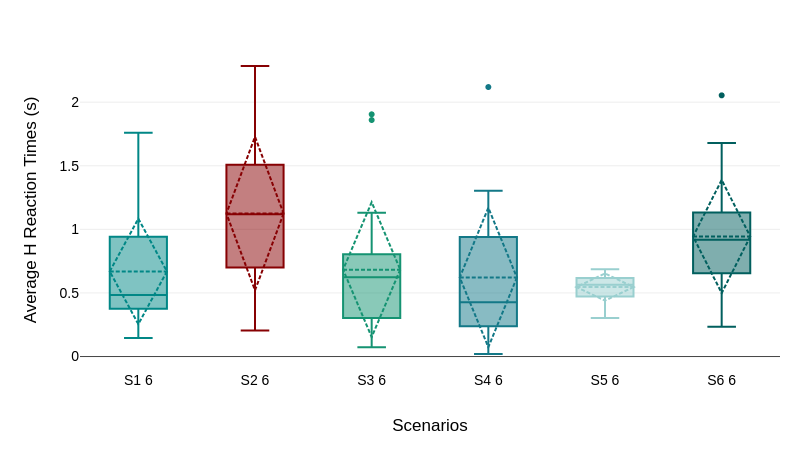
\includegraphics[width=\linewidth]{images/Chapter5/av_reaction_times.png}
    \caption{Average reaction times. For all 6 scenarios. HF has odd numbers, and RF has even numbers. The horizontal dotted line represents the mean value and the dotted triangles the standard deviation around the average.}
    \label{fig:h_reaction_time}
\end{figure}

The average reaction times are measured as follows. After one participant finished one scenario, we measured their reaction time on each step. To do so, we first consider for each step the time when the step begins, which is signaled with text, a gaze and a sound from the robot. Then we consider the time when the human sends a signal by either starting an action or by waving their hand. The duration between these two times is considered as the reaction time of the human. Note that if the human remains passive (no signal) for a step, no reaction time is computed for this specific step. Then, we extract the average reaction time of the participant on the scenario from all the computed ones, compute the standard deviation \textit{and get the maximum and minimum values.}

Average reaction over all scenarios is about $0.76s$. Max values : ?

The ANOVA indicates that the only significant differences are between S2-S5 and S5-S6. 
Indeed, S2 is the RF robot with a correct estimation of human preferences. Since the robot takes the lead people tend to follow the robot and pay attention to what it is doing, not only to the scene. Hence, it is longer to process both the scene and the robot action/intentions and the reaction time tend 

\subsection*{H waiting for the robot (passive, tps mort)}

\subsection*{Tps execution actions}

\subsection*{Combien de fois dépasse TO?}
\textbf{TODO: hard to measure actually... Would be easy to just count number to TO signals. However, with AUTO-PASS TO are triggered anyway, and which shouldn't be counted as TO.}

\subsection{From questionnaires}

Statistical significance. It has been commonly assumed that a statistical test demonstrates a significant difference if a p value lower than $0.05$ is obtained. However, obtaining a value lower than $0.001$ is desired. To make the p values more legible the following standard notation has been adopted:

\begin{align*}
    p > 0.05        & \Rightarrow ns ~ (\textrm{non significant})\\
    p \leq 0.05     & \Rightarrow * ~ (\textrm{significant})\\
    p \leq 0.01     & \Rightarrow ** ~ (\textrm{very significant})\\
    p \leq 0.001    & \Rightarrow *** ~ (\textrm{highly significant})\\
\end{align*}

Some questions have large standard deviations, such as about the perceived ``Intelligence'', but often only on specific scenarios.

The ``Reactive'' answers are overall the same, whatever execution regime and scenario. 
Overall, based on an ANalysis Of the VAriance with repeated measures (ANOVA), all other answers than ``Reactive'' vary significantly. Post-tests show that the main differences come from scenarios S4 and S6. Those two scenarios correspond to ones where the robot has an incorrect estimation of the human preferences and is following the \textit{Robot-First} execution regime. This indicates that all HF behaviors are perceived similarly despite the erroneous estimation of the robot. It also indicates that the RF scenario with correct estimation is positively perceived, but an erroneous estimation has a significant impact on the answers when using RF.  

Except for the ``Reactive'' aspect, answers about RF have a larger standard deviation. Thus, participants tend to be more indecisive regarding RF than HF.

About ``Reactive''. A Bonferroni Post hoc test was used to compare the groups in pairs to find out which was significantly different.
Despite the significant difference in the ANOVA, no pairwise group comparison was significant in the Bonferroni Post hoc test; all p values were greater than 0,05. 

S4 and S6 received significantly worse answers than the other scenarios. It is interesting to notice that in a pair-wise manner, all other scenarios 

We notice very few significant differences on HF only.

\begin{figure}
    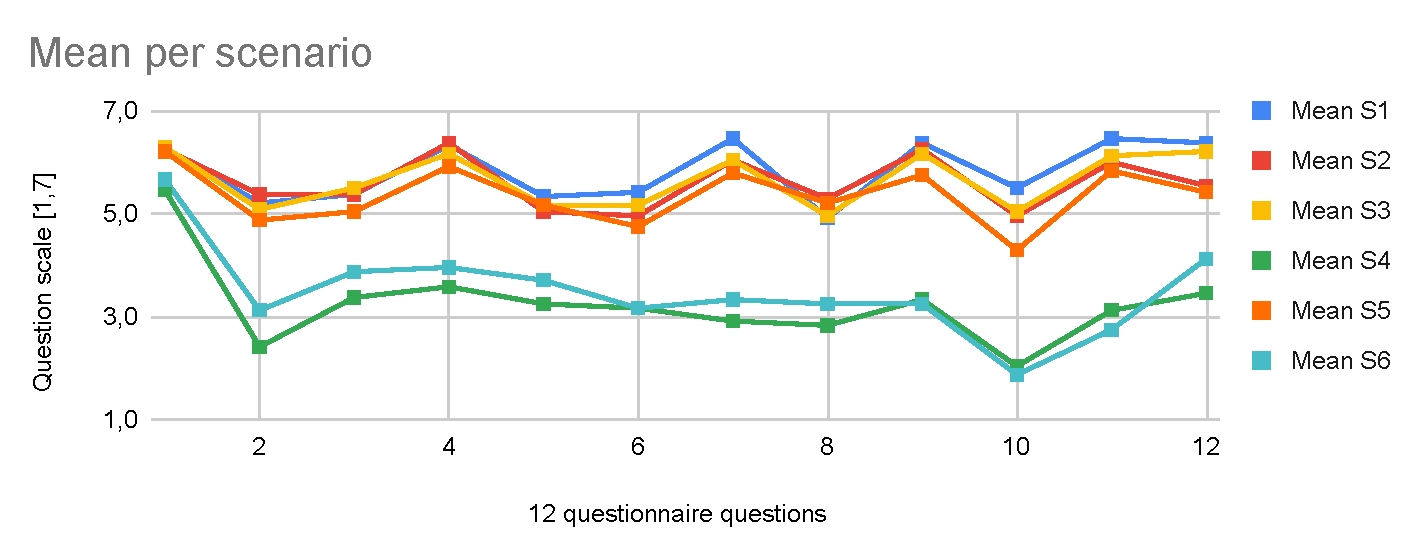
\includegraphics[width=\linewidth]{images/Chapter5/Mean per scenario.pdf}
    \caption{Average value of each question w.r.t. each scenario. S4 and S6 have distinguishable lower values than the other scenarios. We can also notice that the HF scenarios and the RF scenario with correct estimation (2) have roughly the same quite positive answers.}
    \label{fig:mean_per_scenario}
\end{figure}

\begin{figure}
    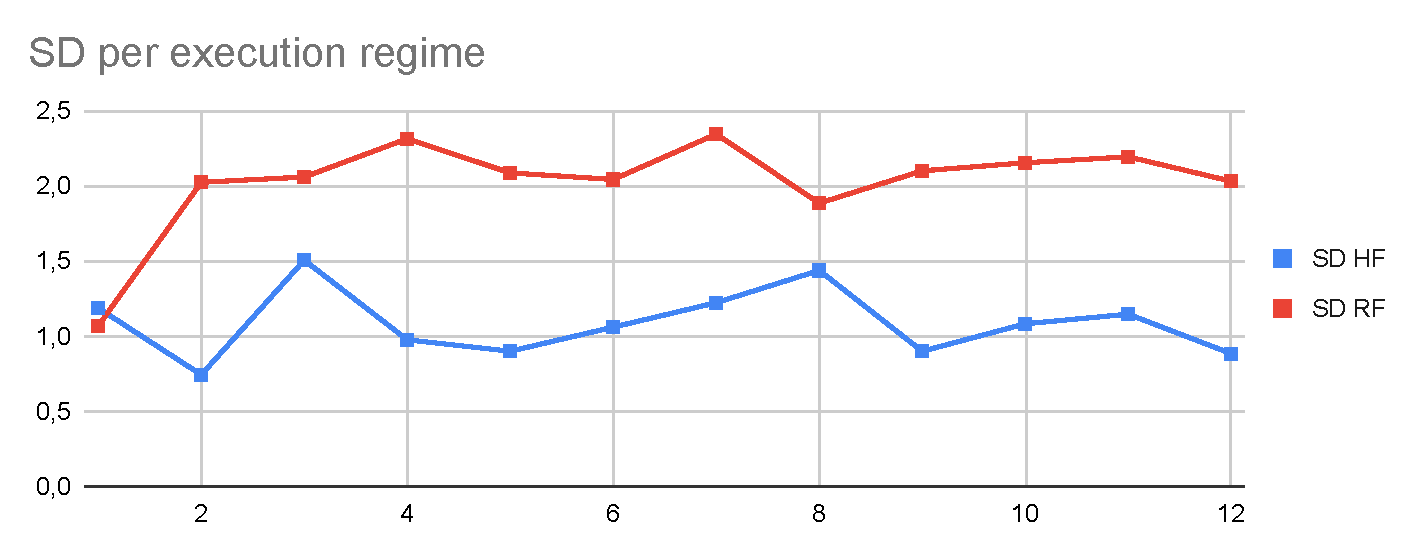
\includegraphics[width=\linewidth]{images/Chapter5/SD per execution regime.pdf}
    \caption{Standard Deviation for each question w.r.t. to all HF scenarios and all RF scenarios. Overall, answers fluctuate more for RF scenarios than with HF.}
    \label{fig:sd_per_execution_regime}
\end{figure}

\begin{figure}
    \centering
    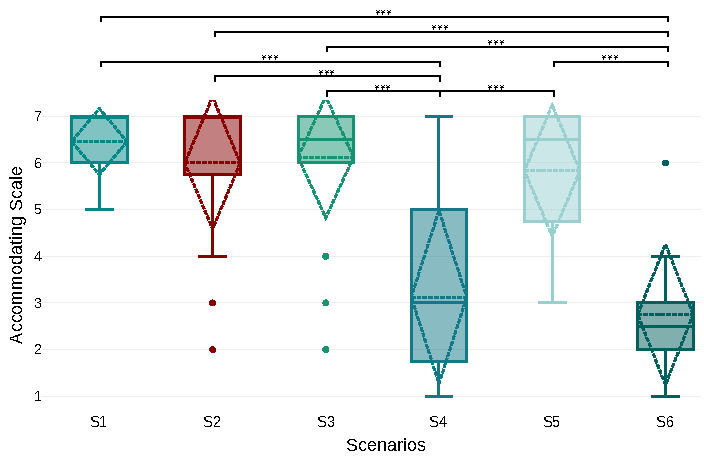
\includegraphics[width=\linewidth]{images/Chapter5/signif_accommo.pdf}
    \caption{Accommodating Interaction Scale with ANOVA + Post-hoc-Tests}
    \label{fig:accommodating_scale_anova}
\end{figure}

% \begin{figure}
%     \centering
%     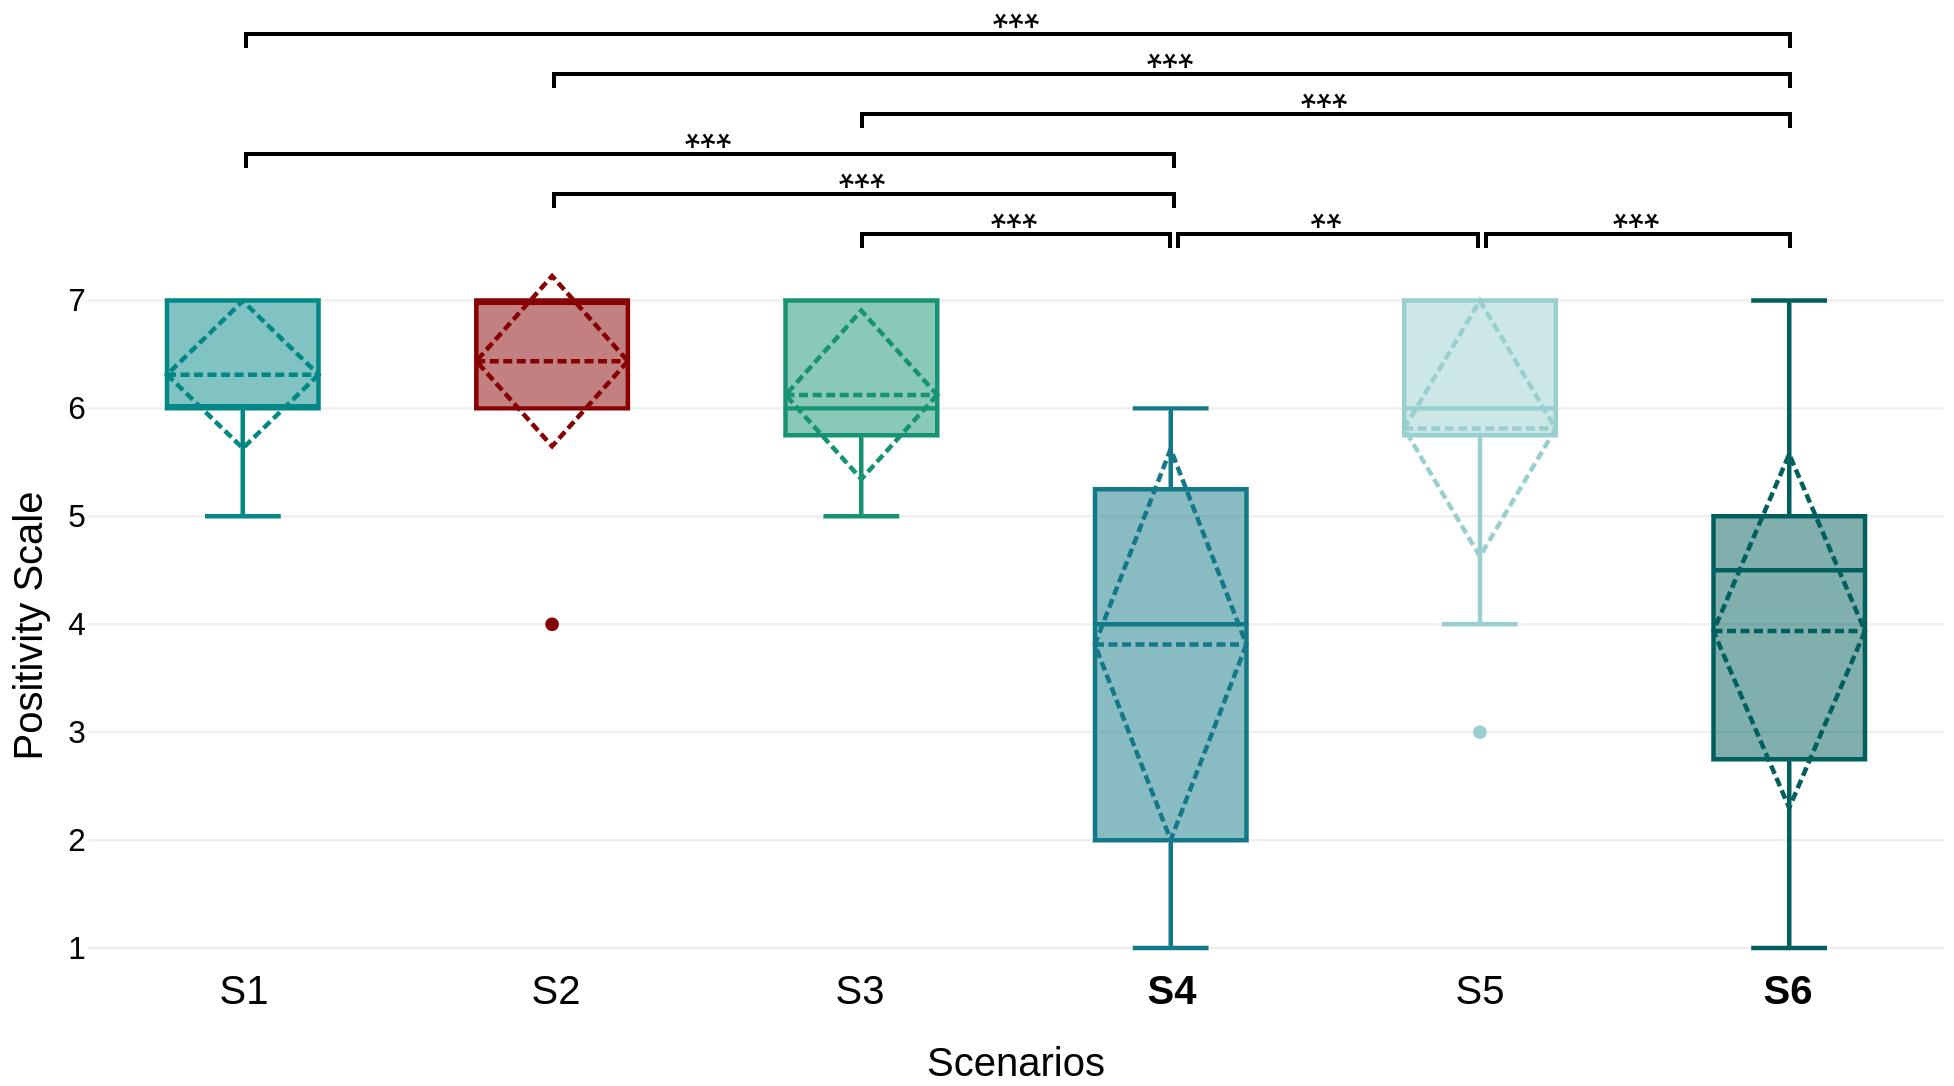
\includegraphics[width=\linewidth]{images/Chapter5/positive_scale.png}
%     \caption{Positive Interaction Scale with ANOVA + Post-hoc-Tests}
%     \label{fig:positive_scale_anova}
% \end{figure}

% \begin{figure}
%     \centering
%     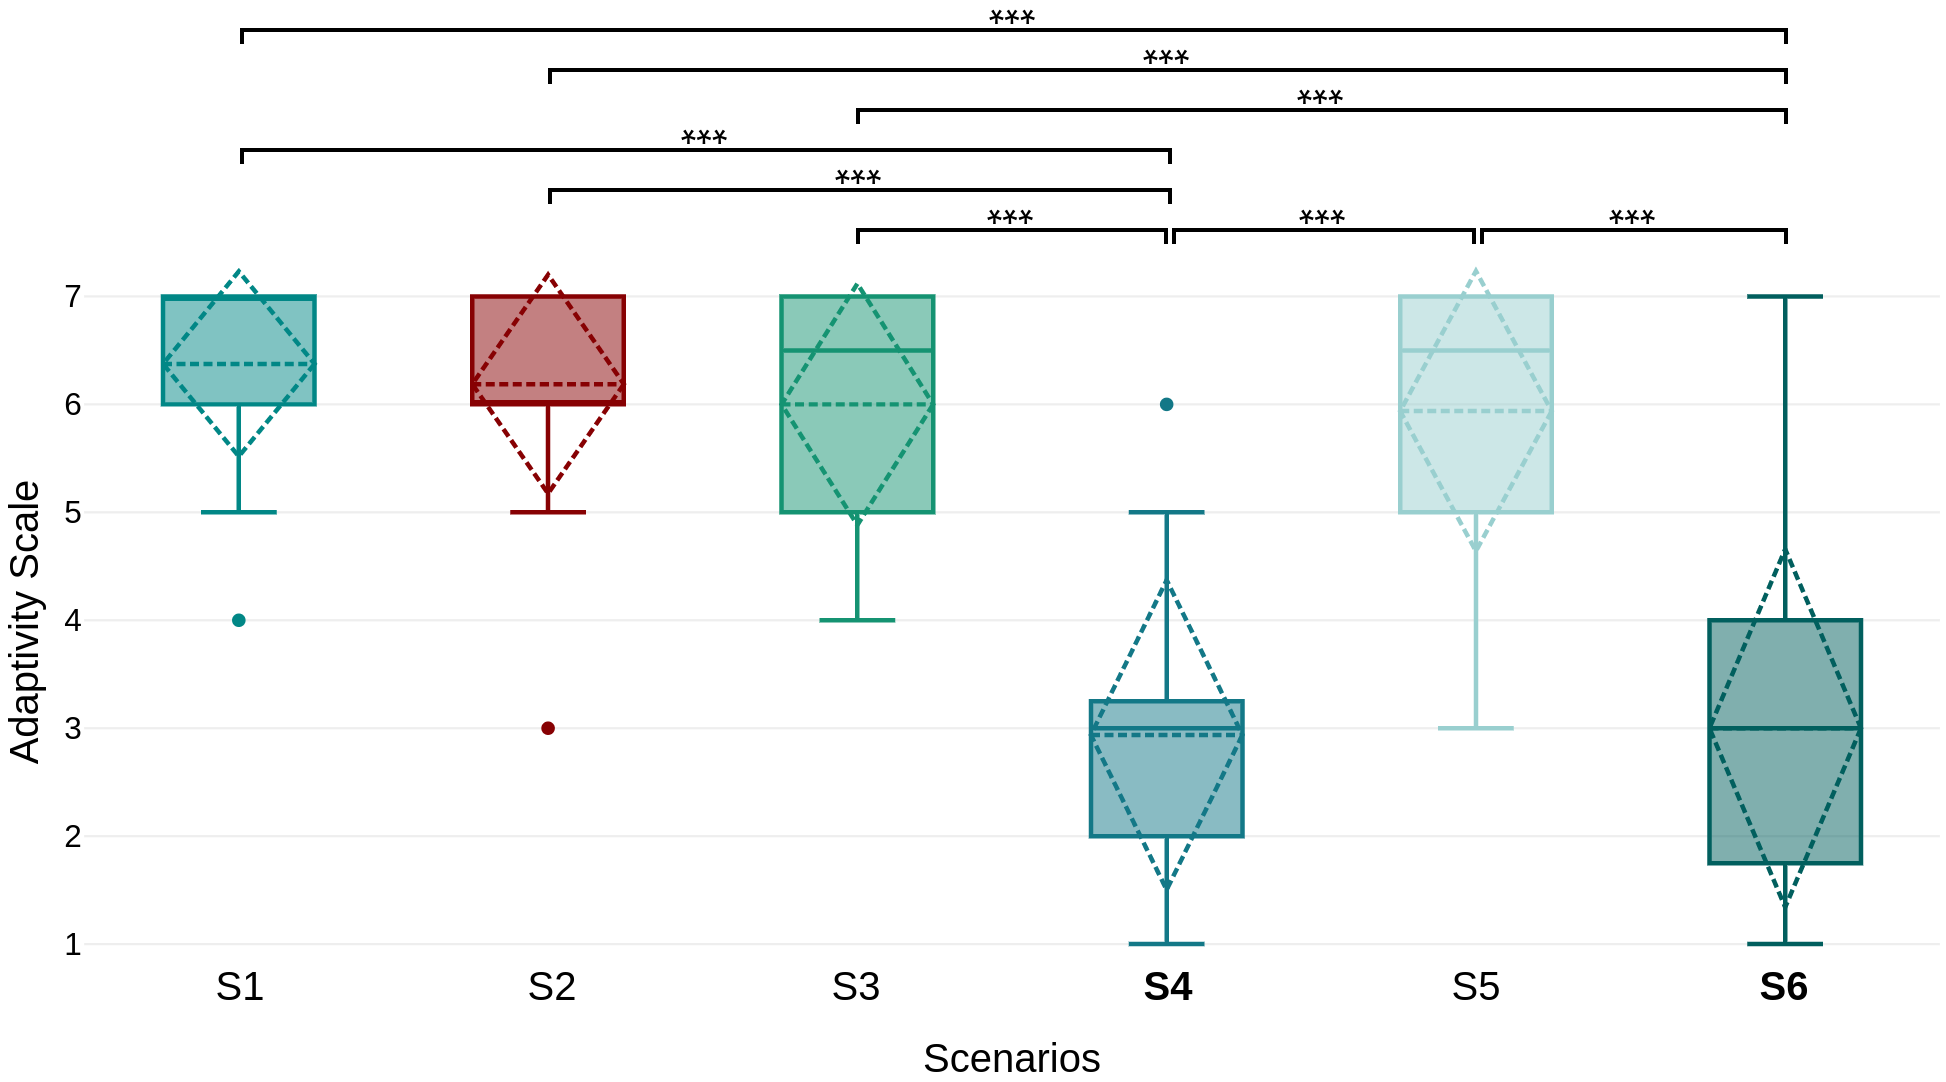
\includegraphics[width=\linewidth]{images/Chapter5/adaptivity_scale.png}
%     \caption{Adaptivity Scale with ANOVA + Post-hoc-Tests}
%     \label{fig:adaptivity_scale_anova}
% \end{figure}


% \begin{table}[]
%     \begin{tabular}{c|c|c|c|c|c|c|c|c|c|c|c}
%     \cline{2-11}
%                                                  & p            & $\eta^2$               & 4-1          & 4-2          & 4-3          & 4-5          & 6-1          & 6-2          & 6-3          & 6-5          &           \\ \cline{1-11}
%     \multicolumn{1}{|c|}{Responsive}             & \textit{***} & \textit{0,16}          & \textit{ns}  & \textit{ns}  & \textit{ns}  & \textit{ns}  & \textit{ns}  & \textit{ns}  & \textit{ns}  & \textit{ns}  & \textit{} \\ \cline{1-11}
%     \multicolumn{1}{|c|}{Competent}              & \textit{***} & \textit{0,49}          & \textit{***} & \textit{***} & \textit{***} & \textit{***} & \textit{***} & \textit{***} & \textit{**}  & \textit{*}   & \textit{} \\ \cline{1-11}
%     \multicolumn{1}{|c|}{Intelligent}            & \textit{***} & \textit{0,33}          & \textit{**}  & \textit{**}  & \textit{**}  & \textit{*}   & \textit{*}   & \textit{*}   & \textit{***} & \textit{*}   & \textit{} \\ \cline{1-11}
%     \multicolumn{1}{|c|}{\textbf{Positive}}      & \textit{***} & \textit{\textbf{0,64}} & \textit{***} & \textit{***} & \textit{***} & \textit{***} & \textit{***} & \textit{***} & \textit{***} & \textit{***} & \textit{} \\ \cline{1-11}
%     \multicolumn{1}{|c|}{Simple}                 & \textit{***} & \textit{0,33}          & \textit{**}  & \textit{*}   & \textit{*}   & \textit{**}  & \textit{*}   & \textit{ns}  & \textit{*}   & \textit{*}   & \textit{} \\ \cline{1-11}
%     \multicolumn{1}{|c|}{Clear}                  & \textit{***} & \textit{0,41}          & \textit{***} & \textit{**}  & \textit{**}  & \textit{*}   & \textit{***} & \textit{**}  & \textit{**}  & \textit{*}   & \textit{} \\ \cline{1-11}
%     \multicolumn{1}{|c|}{\textbf{Adaptive}}      & \textit{***} & \textit{\textbf{0,62}} & \textit{***} & \textit{***} & \textit{***} & \textit{***} & \textit{***} & \textit{***} & \textit{***} & \textit{***} & \textit{} \\ \cline{1-11}
%     \multicolumn{1}{|c|}{Useful}                 & \textit{***} & \textit{0,43}          & \textit{**}  & \textit{***} & \textit{***} & \textit{***} & \textit{*}   & \textit{***} & \textit{**}  & \textit{***} & \textit{} \\ \cline{1-11}
%     \multicolumn{1}{|c|}{\textbf{Efficient}}     & \textit{***} & \textit{\textbf{0,61}} & \textit{***} & \textit{***} & \textit{***} & \textit{***} & \textit{***} & \textit{***} & \textit{***} & \textit{***} & \textit{} \\ \cline{1-11}
%     \multicolumn{1}{|c|}{\textbf{Appropriate}}   & \textit{***} & \textit{\textbf{0,6}}  & \textit{***} & \textit{***} & \textit{***} & \textit{**}  & \textit{***} & \textit{***} & \textit{***} & \textit{***} & \textit{} \\ \cline{1-11}
%     \multicolumn{1}{|c|}{\textbf{Accommodating}} & \textit{***} & \textit{\textbf{0,67}} & \textit{***} & \textit{***} & \textit{***} & \textit{***} & \textit{***} & \textit{***} & \textit{***} & \textit{***} & \textit{} \\ \cline{1-11}
%     \multicolumn{1}{|c|}{Predictable}            & \textit{***} & \textit{0,44}          & \textit{***} & \textit{**}  & \textit{***} & \textit{*}   & \textit{***} & \textit{*}   & \textit{***} & \textit{**}  & \textit{} \\ \cline{1-11}
%     \end{tabular}
%     \caption{Significant differences in the questionnaire answers between the different scenarios. For each item of the questionnaire are shown the overall p value and $\eta^2$ (effect size) obtained after an ANOVA. Additionally, the p values obtained after conducting Bonferroni Post-hoc-Tests are shown to identify which in a pair-wise manner which scenario were significantly different from others. As depicted, the scenarios 4 and 6 are distinguishable from the others and their evaluation are significantly different on all the measured aspect (expect reactivity).}
%     \label{tab:questionnaire_answers}
% \end{table}


\begin{sidewaystable}
    \center
        \begin{tabular}{c|c|c|c|c|c|c|c|c|c|c|c|c|c|c|c|c|c|}
        \cline{2-18}
        \multicolumn{1}{l|}{}                       & p   & d             & 1-2 & 1-3 & \textbf{1-4} & 1-5 & \textbf{1-6} & 2-3 & \textbf{2-4} & 2-5 & \textbf{2-6} & \textbf{3-4} & 3-5 & \textbf{3-6} & \textbf{4-5} & \textbf{4-6} & \textbf{5-6} \\ \hline
        \multicolumn{1}{|c|}{Réactivité}            & *** & 0,16          & ns  & ns  & ns           & ns  & ns           & ns  & ns           & ns  & ns           & ns           & ns  & ns           & ns           & ns           & ns           \\ \hline
        \multicolumn{1}{|c|}{Compétent}             & *** & 0,49          & ns  & ns  & ***          & ns  & ***          & ns  & ***          & ns  & ***          & ***          & ns  & **           & ***          & ns           & *            \\ \hline
        \multicolumn{1}{|c|}{Intelligence}          & *** & 0,33          & ns  & ns  & **           & ns  & *            & ns  & **           & ns  & *            & **           & ns  & ***          & *            & ns           & *            \\ \hline
        \multicolumn{1}{|c|}{\textbf{Positive}}     & *** & \textbf{0,64} & ns  & ns  & ***          & ns  & ***          & ns  & ***          & ns  & ***          & ***          & ns  & ***          & ***          & ns           & ***          \\ \hline
        \multicolumn{1}{|c|}{Simple}                & *** & 0,33          & ns  & ns  & **           & ns  & *            & ns  & *            & ns  & ns           & *            & ns  & *            & **           & ns           & *            \\ \hline
        \multicolumn{1}{|c|}{Clair}                 & *** & 0,41          & ns  & ns  & ***          & ns  & ***          & ns  & **           & ns  & **           & **           & ns  & **           & *            & ns           & *            \\ \hline
        \multicolumn{1}{|c|}{\textbf{Adaptativité}} & *** & \textbf{0,62} & ns  & ns  & ***          & ns  & ***          & ns  & ***          & ns  & ***          & ***          & ns  & ***          & ***          & ns           & ***          \\ \hline
        \multicolumn{1}{|c|}{Utile}                 & *** & 0,43          & ns  & ns  & **           & ns  & *            & ns  & ***          & ns  & ***          & ***          & ns  & **           & ***          & ns           & ***          \\ \hline
        \multicolumn{1}{|c|}{\textbf{Efficacité}}   & *** & \textbf{0,61} & ns  & ns  & ***          & ns  & ***          & ns  & ***          & ns  & ***          & ***          & ns  & ***          & ***          & ns           & ***          \\ \hline
        \multicolumn{1}{|c|}{\textbf{Adéquat}}      & *** & \textbf{0,6}  & ns  & ns  & ***          & **  & ***          & ns  & ***          & ns  & ***          & ***          & ns  & ***          & **           & ns           & ***          \\ \hline
        \multicolumn{1}{|c|}{\textbf{Accommodant}}  & *** & \textbf{0,67} & ns  & ns  & ***          & ns  & ***          & ns  & ***          & ns  & ***          & ***          & ns  & ***          & ***          & ns           & ***          \\ \hline
        \multicolumn{1}{|c|}{Prévisible}            & *** & 0,44          & ns  & ns  & ***          & **  & ***          & ns  & **           & ns  & *            & ***          & *   & ***          & *            & ns           & **           \\ \hline
        \end{tabular}
    \caption{Significant differences in the questionnaire answers between the different scenarios. For each item of the questionnaire are shown the overall p value and $\eta^2$ (effect size) obtained after an ANOVA. Additionally, the p values obtained after conducting Bonferroni Post-hoc-Tests are shown to identify which in a pair-wise manner which scenario were significantly different from others. As depicted, the scenarios 4 and 6 are distinguishable from the others and their evaluation are significantly different on all the measured aspect (expect reactivity).}
    \label{tab:questionnaire_answers}
\end{sidewaystable}

\begin{table}[]
    \footnotesize
    \begin{tabular}{ccc}
    \hline
    \textbf{Dimension}                         & \textbf{Question}                                                                                                                     & \textbf{Item}             \\ \hline
    \multirow{3}{*}{\textbf{Robot perception}} & \multirow{3}{*}{\begin{tabular}[c]{@{}c@{}}In your opinion,\\ the robot is rather:\end{tabular}}                                      & Apathetic/Responsive      \\
                                               &                                                                                                                                       & Incompetent/Competent     \\
                                               &                                                                                                                                       & Unintelligent/Intelligent \\ \hline
    \multirow{3}{*}{\textbf{Interaction}}      & \multirow{3}{*}{\begin{tabular}[c]{@{}c@{}}In your opinion, the interaction\\ with the robot was:\end{tabular}}                       & Negative/Positive         \\
                                               &                                                                                                                                       & Complicated/Simple        \\
                                               &                                                                                                                                       & Ambiguous/Clear           \\ \hline
    \multirow{3}{*}{\textbf{Collaboration}}    & \multirow{3}{*}{\begin{tabular}[c]{@{}c@{}}In your opinion, the collaboration\\ with the robot to perform the task was:\end{tabular}} & Restrictive/Adaptive      \\
                                               &                                                                                                                                       & Useless/Useful            \\
                                               &                                                                                                                                       & Inefficient/Efficient     \\ \hline
    \multirow{3}{*}{\textbf{Acting}}           & \multirow{3}{*}{\begin{tabular}[c]{@{}c@{}}In your opinion, the robot\\ choices of action were:\end{tabular}}                         & Inappropriate/Appropriate \\
                                               &                                                                                                                                       & Annoying/Accommodating    \\
                                               &                                                                                                                                       & Unpredictable/Predictable \\ \hline
    \end{tabular}
    \caption{PeRDITA Questionnaire: Participants have to place themselves between the two antonym items in a scale of 7.}
    \label{tab:perdita_questionnaire}
\end{table}

\section{Discussion}

fazfa


\section{Conclusion}

fazfafza